\appendix

\section*{Appendix A: Supplementary Figures}
\addcontentsline{toc}{section}{Appendix A: Supplementary Figures}
\begin{suppfigure}
\includesvg[width=\textwidth]{lab/fluorescense_intensity.svg}
\caption{\textbf{Calibration curve for the estimation of Strep-eYFP yield in the ALiCE reaction mix.} The calibration samples were created by diluting purified Strep-eYFP in PBS. The measurements for the highest two concentrations were left out when fitting the linear model, since they are far beyond the fluorescence measured in the samples. The measurement data can be found in \autoref{tab:calibration_values_eyfp}. }
\label{fig:calibration_eyfp}
\end{suppfigure}

\begin{suppfigure}
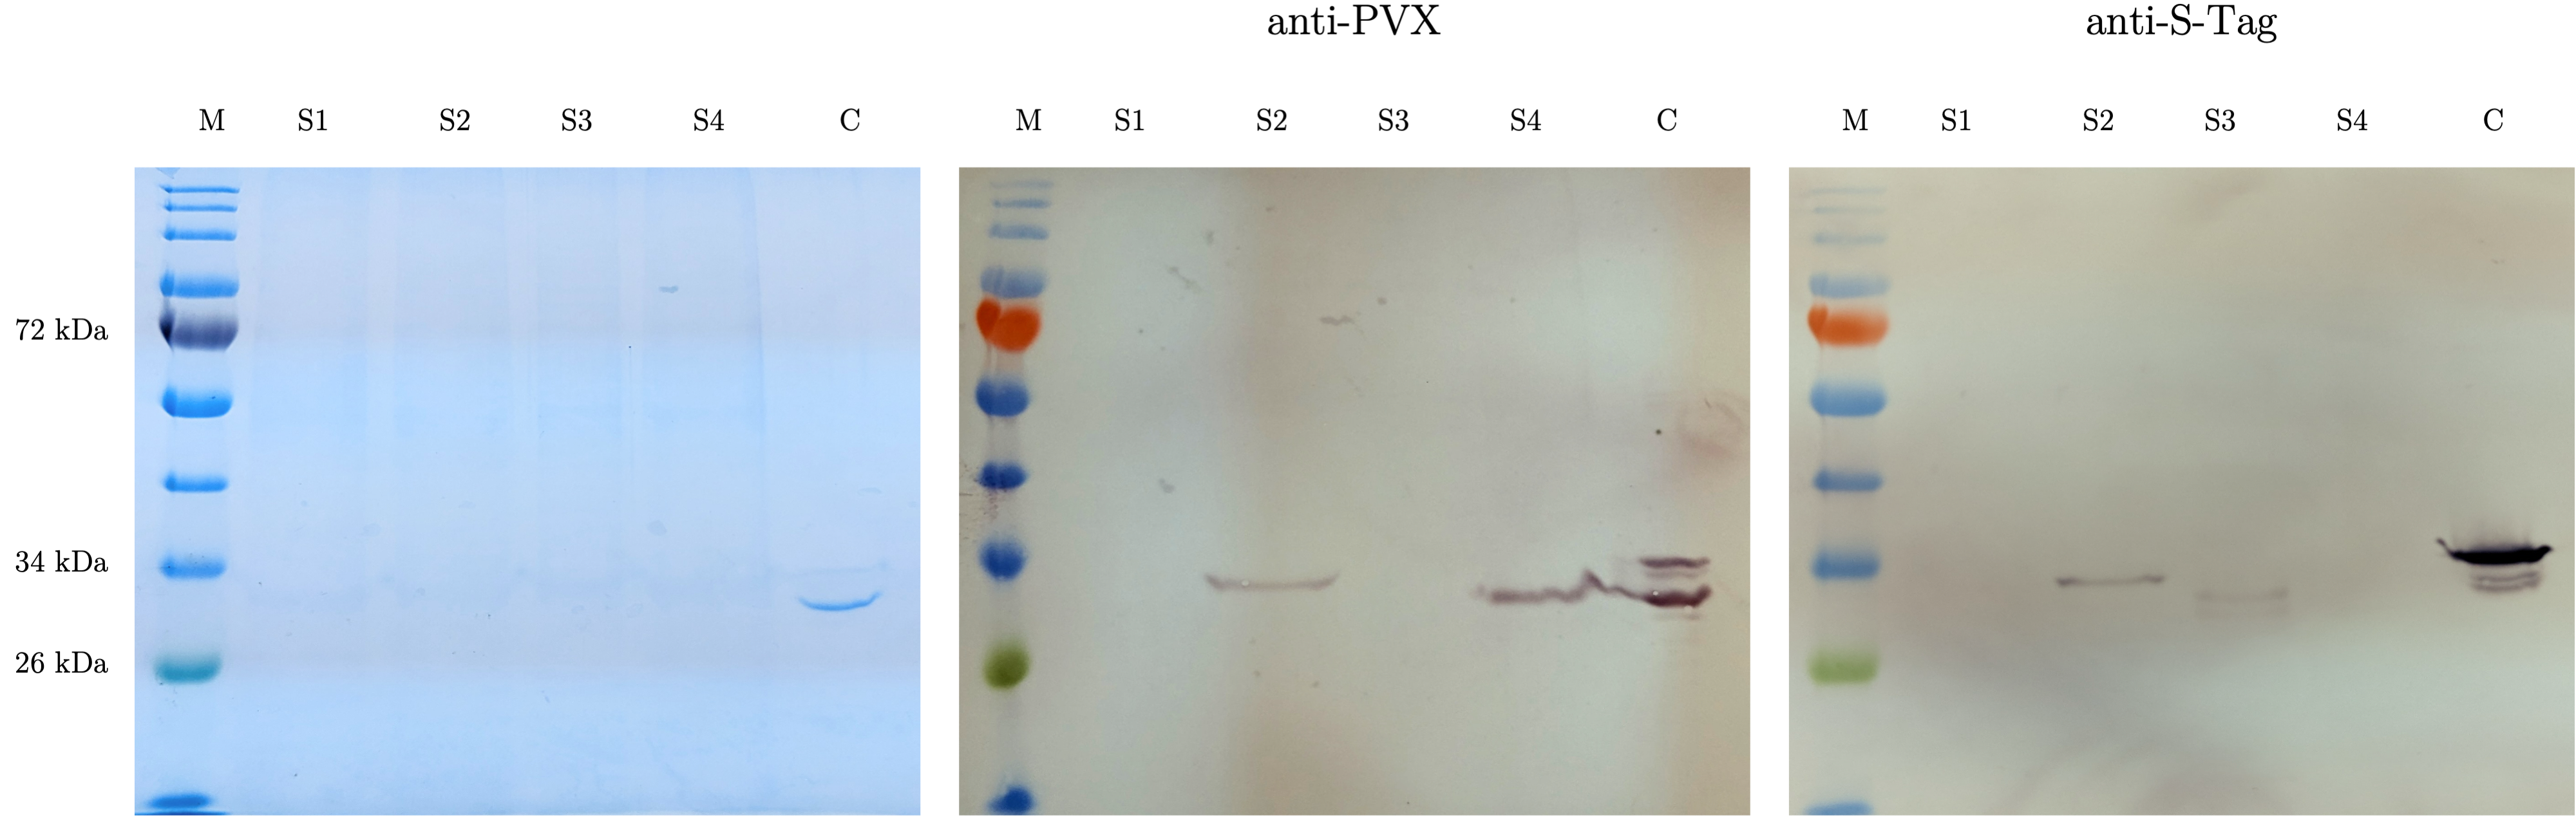
\includegraphics{lab/blot_capto.png}
\caption{\textbf{Initial Coomassie Gel and Western Blot images following CaptoCore Purification.} The samples showed a precipitate, possibly resin from the chromatography column. Samples were taken from the concentrated CaptoCore flow-through for the constructs d29-A (S1), S-Tag-A (S2), S-Tag-B (S3), and PVX CP (S4). S-Tag-PVX virons were used as control (C1). The marker was NEB Color Prestained Protein Standard, Broad Range (10-250 kDa). The Western Blot using the anti-PVX antibody showed signals for S-Tag-A, PVX CP, and the control. The Western Blot based on the anti-S-Tag antibody showed signals for S-Tag-A and the control, as well as a faint signal for S-Tag-B. }
\label{fig:blot_capto}
\end{suppfigure}

\begin{suppfigure}
\includesvg[width=\textwidth]{lab/elisa_calibration.svg}
\caption{\textbf{Calibration curves of the ELISA after cell-free expression. } Two assays were conducted, using both the anti-PVX antibody and the anti-S-Tag antibody. The calibration samples were created by diluting S-Tag-PVX virions in coating buffer. Only the data points of the lowest four concentrations were used in the estimation of the linear model for the anti-PVX antibody, because the data showed saturation. }
\label{fig:elisa_calib}
\end{suppfigure}

\begin{suppfigure}
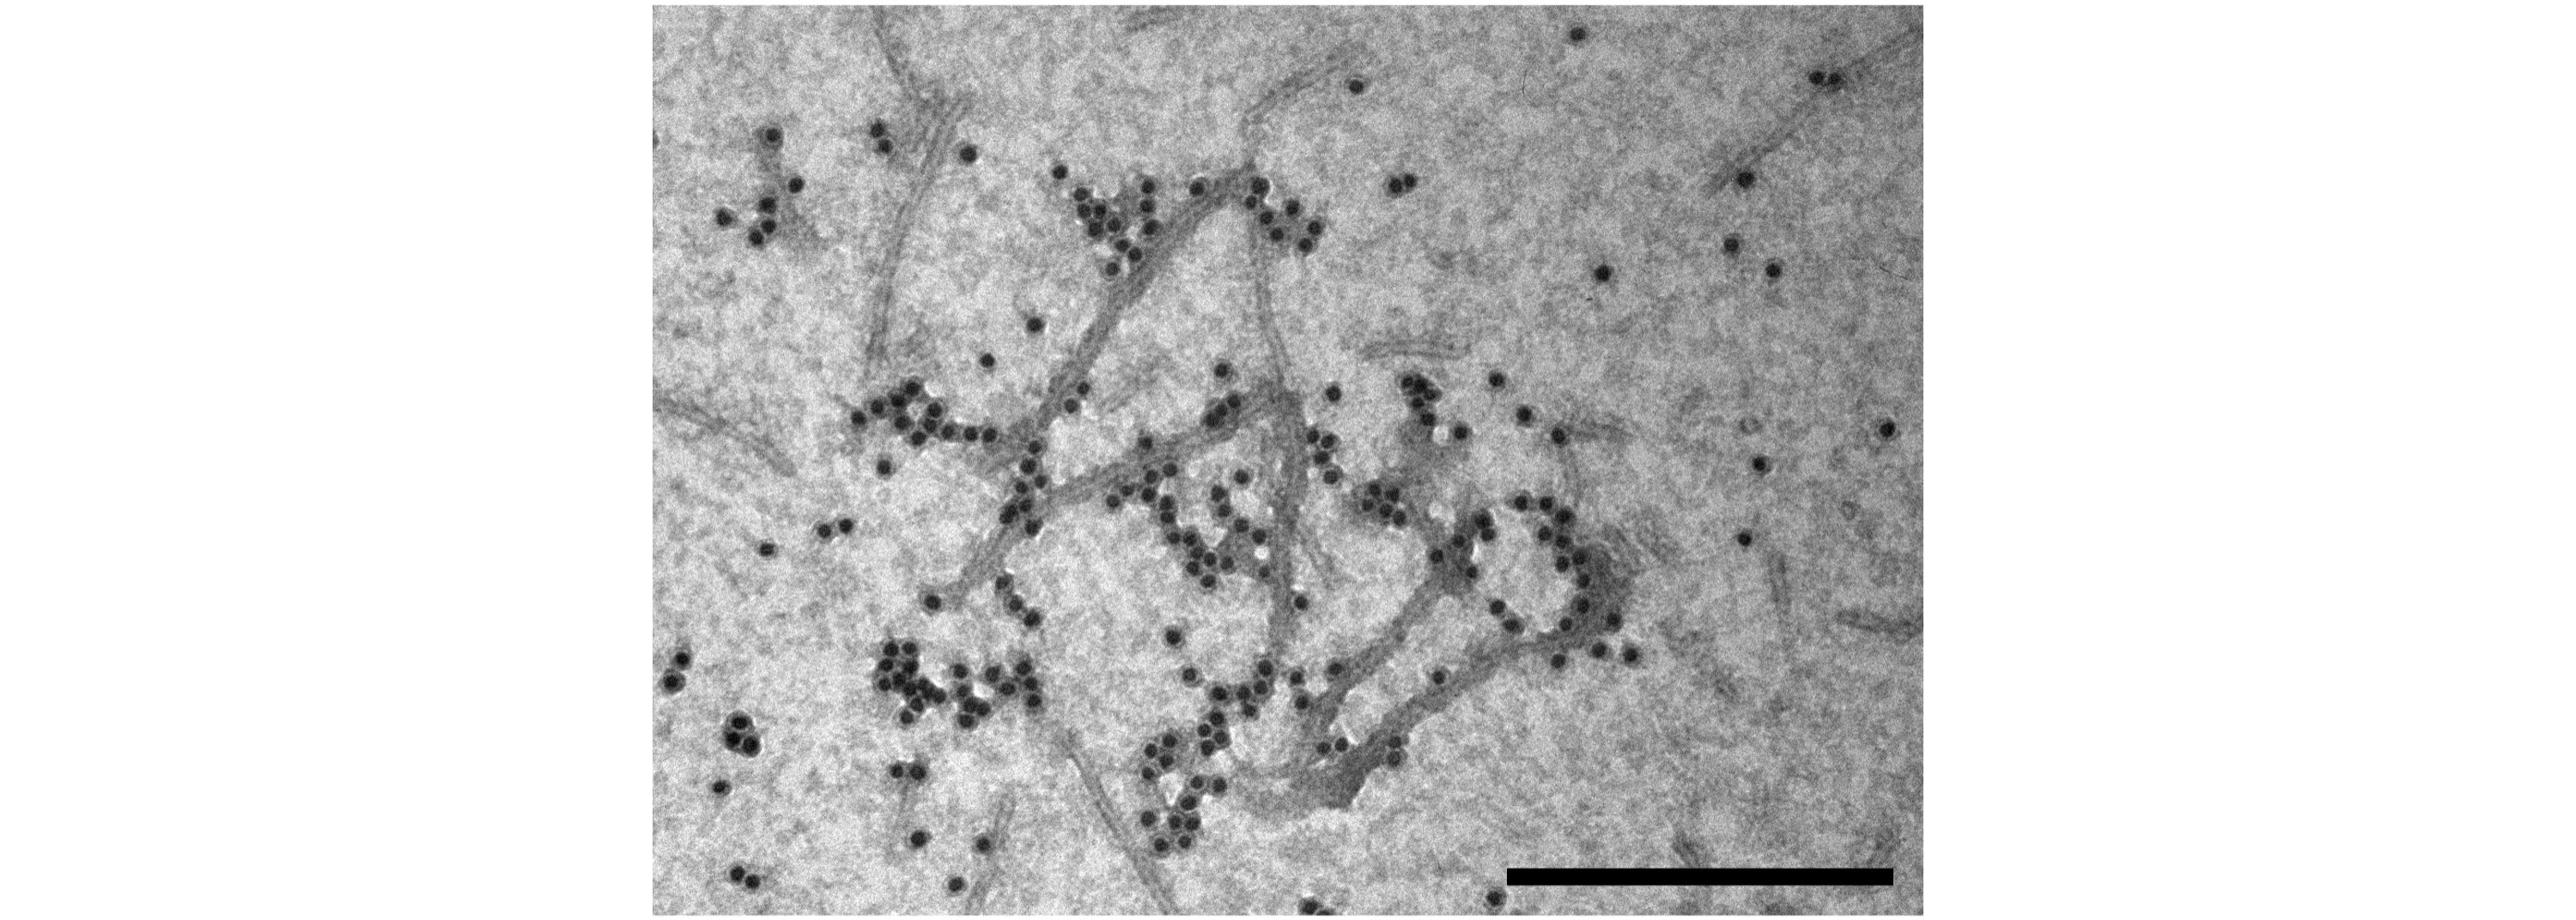
\includegraphics{lab/em_immuno_labeling.png}
\caption{\textbf{Examplary TEM Image of Immunogold labeling of S-Tag-PVX virions. } The image was provided by the Institute for Molecular Biotechnology. The particles were purified from plant infection, captured using an anti-PVX antibody and labeled using a mouse-anti-S-Tag antibody and a gold-conjugated goat-anti-mouse antibody. }
\label{fig:em_immuno_labeling}
\end{suppfigure}

\section*{Appendix B: Supplementary Tables}
\addcontentsline{toc}{section}{Appendix B: Supplementary Tables}

\begin{supptable}[ht]
    \centering
    \caption{\textbf{Calibration data for the estimation of Strep-eYFP yield in the ALiCE reaction mix.} The calibration samples were created by diluting purified Strep-eYFP in PBS. A visualization of the data and a linear model fitted against it can be found in \autoref{fig:calibration_eyfp}.}\label{tab:calibration_values_eyfp}
    \begin{tabular}{S[table-format=3.1] S[table-format=5.0(4), uncertainty-mode=separate]}
    \toprule
    {Concentration (\si{\micro\gram\per\milli\litre})} & {Fluorescence } \\
    \midrule
    100.0 & 38253(1972) \\
    50.0  & 20639(618) \\
    25.0  & 9445(388) \\
    10.0  & 3049(181) \\
    5.0   & 1078(56) \\
    2.5   & 405(18) \\
    \bottomrule
    \end{tabular}
\end{supptable}

\begin{supptable}[ht]
    \centering
    \caption{\textbf{Measured fluorescence and estimated eYFP concentrations for Strep-eYFP (ALiCE) and Non-template (ALiCE). } The concentration was calculated from the fluorescence using the linear model shown in \autoref{fig:calibration_eyfp}. Back-calculation of the original sample concentration was done by multiplication with the dilution factor. }
    \label{tab:sample_values_eyfp}
    \begin{tabular}{
        l
        S[table-format=4.0(2),uncertainty-mode = separate]
        S[table-format=1.2(2),uncertainty-mode = separate]
        S[table-format=3.1(2),uncertainty-mode = separate]
    }
    \toprule
    {\textbf{Dilution}} &
    {\textbf{Fluorescence}} &
    {\textbf{Conc. (\si{\micro\gram\per\milli\litre})}} &
    {\textbf{Back-calculated (\si{\micro\gram\per\milli\litre})}} \\
    \midrule
    \multicolumn{2}{l}{\textbf{Strep-eYFP (ALiCE)}} \\
    1:50   & 2149(87)   & 5.95(0.24) & 298(12) \\
    1:100  & 1107(47)   & 3.07(0.13) & 307(13) \\
    1:200  & 505 (42)    & 1.40(0.12) & 280(23) \\
    1:500  & 184 (3)    & 0.51(0.01) & 255(5) \\
    \midrule
    \multicolumn{2}{l}{\textbf{Non-template (ALiCE)}} \\
    1:50   & 1(1)       & 0.00(0.00) & 0(0.1) \\
    1:100  & -1(0)      & 0.00(0.00) & 0(0.0) \\
    1:200  & 0(1)      & 0.00(0.00) & 0(0.3) \\
    1:500  & -1(1)      & 0.00(0.00) & -1(0.8) \\
    \bottomrule
    \end{tabular}
\end{supptable}

\begin{supptable}[ht]
    \centering
    \caption{\textbf{Calibration data of the ELISA after cell-free expression. } Two assays were conducted, using both the anti-PVX antibody and the anti-S-Tag antibody. The calibration samples were created by diluting S-Tag-PVX virions in coating buffer. A visualization of the data and a linear model fitted against it can be found in \autoref{fig:elisa_calib}.}
    \label{tab:calibration_data_elisa}
    \begin{tabular}{
        S[table-format=4.0]
        S[table-format=1.3(3),uncertainty-mode=separate]
        S[table-format=1.3(3),uncertainty-mode=separate]
    }
    \toprule
    {Concentration (\si{\nano\gram\per\milli\litre})} &
    {OD (anti-PVX)} &
    {OD (anti-S-Tag)} \\
    \midrule
    1500 & 2.322(0.037) & 1.474(0.054) \\
    1000 & 1.895(0.067) & 0.847(0.032) \\
    500  & 1.303(0.026) & 0.355(0.021) \\
    250  & 1.003(0.037) & 0.111(0.019) \\
    100  & 0.597(0.031) & 0.017(0.018) \\
    50   & 0.395(0.026) & -0.001(0.017) \\
    25   & 0.224(0.032) & -0.005(0.017) \\
    10   & 0.105(0.026) & 0.009(0.018) \\
    \bottomrule
    \end{tabular}
\end{supptable}

\begin{supptable}[ht]
    \centering
    \caption{\textbf{Measured OD and estimated antigen concentrations for the ELISA using the anti-PVX antibody.} The concentration was calculated from the OD using the linear model discussed in \autoref{subsection:elisa} and multiplication with the dilution factor. }
    \label{tab:sample_values_elisa_anti_pvx}
    \begin{tabular}{
        l
        S[table-format=1.3(2),uncertainty-mode=separate]
        S[table-format=3.1(1),uncertainty-mode=separate]
    }
    \toprule
    {\textbf{Sample (Dilution)}} &
    {\textbf{OD}} &
    {\textbf{Back-calculated (\si{\micro\gram\per\milli\litre})}} \\
    \midrule
    \textbf{d29-A} \\
    1:500 & 0.208(0.028) & 16.0(2.2) \\
    1:1000 & 0.200(0.032) & 30.7(4.9) \\
    \textbf{S-Tag-A} \\
    1:500 & 0.234(0.033) & 18.0(2.5) \\
    1:1000 & 0.217(0.026) & 33.4(4.0) \\
    \textbf{S-Tag-B} \\
    1:500 & 0.005(0.026) & 0.4(2.0) \\
    1:1000 & 0.020(0.030) & 3.1(4.6) \\
    \textbf{PVX CP} \\
    1:500 & 0.871(0.028) & 66.9(2.2) \\
    1:1000 & 0.873(0.026) & 134.2(4.0) \\
    \textbf{Non-template} \\
    1:500 & 0.036(0.032) & 2.8(2.5) \\
    1:1000 & 0.012(0.040) & 1.9(6.2) \\
    \bottomrule
    \end{tabular}
\end{supptable}

\begin{supptable}[ht]
    \centering
    \caption{\textbf{Measured OD and estimated antigen concentrations for the ELISA using the anti-S-Tag antibody.} The concentration was calculated from the OD using the linear model discussed in \autoref{subsection:elisa} and multiplication with the dilution factor. }
    \label{tab:sample_values_elisa_anti_s_tag}
    \begin{tabular}{
        l
        S[table-format=1.3(2),uncertainty-mode=separate]
        S[table-format=4.0(2),uncertainty-mode=separate]
    }
    \toprule
    {\textbf{Sample (Dilution)}} &
    {\textbf{OD}} &
    {\textbf{Back-calculated (\si{\micro\gram\per\milli\litre})}} \\
    \midrule
    \textbf{d29-A} \\
    1:500 & 0.041(0.023) & 22(12) \\
    1:1000 & 0.041(0.020) & 44(22) \\
    \textbf{S-Tag-A} \\
    1:500 & 2.406(0.134) & 1317(73) \\
    1:1000 & 2.191(0.079) & 2399(86) \\
    \textbf{S-Tag-B} \\
    1:500 & 1.484(0.073) & 813(40) \\
    1:1000 & 1.094(0.098) & 1198(107) \\
    \textbf{PVX CP} \\
    1:500 & 0.022(0.018) & 12(10) \\
    1:1000 & 0.046(0.020) & 50(22) \\
    \textbf{Non-template} \\
    1:500 & 0.039(0.018) & 21(10) \\
    1:1000 & 0.036(0.019) & 38(21) \\
    \bottomrule
    \end{tabular}
\end{supptable}

%\begin{supptable}[ht]
%    \centering
%    \caption{Estimated concentrations from anti-PVX ELISA}
%    \begin{tabular}{
%        l
%        S[table-format=1.3(2),uncertainty-mode=separate]
%        S[table-format=2.2(2),uncertainty-mode=separate]
%        S[table-format=3.2(2),uncertainty-mode=separate]
%    }
%    \toprule
%    {\textbf{Sample (Dilution)}} &
%    {\textbf{OD}} &
%    {\textbf{Conc. (ng/mL)}} &
%    {\textbf{Back-calculated (\si{\micro\gram\per\milli\litre})}} \\
%    \midrule
%    \textbf{d29-A} \\
%    1:500 & 0.208(0.028) & 31.98(4.32) & 15.99(2.16) \\
%    1:1000 & 0.200(0.032) & 30.73(4.93) & 30.73(4.93) \\
%    \textbf{S-Tag-A} \\
%    1:500 & 0.234(0.033) & 35.95(5.08) & 17.97(2.54) \\
%    1:1000 & 0.217(0.026) & 33.35(4.03) & 33.35(4.03) \\
%    \textbf{S-Tag-B} \\
%    1:500 & 0.005(0.026) & 0.77(4.01) & 0.39(2.00) \\
%    1:1000 & 0.020(0.030) & 3.07(4.63) & 3.07(4.63) \\
%    \textbf{CP-PVX} \\
%    1:500 & 0.871(0.028) & 133.83(4.37) & 66.92(2.19) \\
%    1:1000 & 0.873(0.026) & 134.16(4.03) & 134.16(4.03) \\
%    \textbf{Non-template} \\
%    1:500 & 0.036(0.032) & 5.49(4.97) & 2.75(2.49) \\
%    1:1000 & 0.012(0.040) & 1.89(6.22) & 1.89(6.22) \\
%    \bottomrule
%    \end{tabular}
%\end{supptable}

%\begin{supptable}[ht]
    %\centering
    %\caption{Estimated concentrations from anti-S-Tag ELISA}
    %\begin{tabular}{
        %l
        %S[table-format=1.3(2),uncertainty-mode=separate]
        %S[table-format=4.0(2),uncertainty-mode=separate]
        %S[table-format=4.0(2),uncertainty-mode=separate]
    %}
    %\toprule
    %{\textbf{Sample (Dilution)}} &
    %{\textbf{OD}} &
    %{\textbf{Conc. (ng/mL)}} &
    %{\textbf{Back-calculated (\si{\micro\gram\per\milli\litre})}} \\
    %\midrule
    %\textbf{d29-A} \\
    %1:500 & 0.041(0.023) & 45(25) & 22(12) \\
    %1:1000 & 0.041(0.020) & 45(22) & 44(22) \\
    %\textbf{S-Tag-A} \\
    %1:500 & 2.406(0.134) & 2634(147) & 1317(73) \\
    %1:1000 & 2.191(0.079) & 2399(86) & 2399(86) \\
    %\textbf{S-Tag-B} \\
    %1:500 & 1.484(0.073) & 1625(79) & 813(40) \\
    %1:1000 & 1.094(0.098) & 1198(107) & 1198(107) \\
    %\textbf{CP-PVX} \\
    %1:500 & 0.022(0.018) & 24(19) & 12(10) \\
    %1:1000 & 0.046(0.020) & 50(22) & 50(22) \\
    %\textbf{Non-template} \\
    %1:500 & 0.039(0.018) & 42(20) & 21(10) \\
    %1:1000 & 0.036(0.019) & 39(21) & 38(21) \\
    %\bottomrule
    %\end{tabular}
%\end{supptable}

\section*{Appendix C: Algorithms}
\addcontentsline{toc}{section}{Appendix C: Algorithms}
\begin{suppalgorithm}
     \caption{Sample Diffusion\\ A faithful recreation of the diffusion sampling algorithm from the AlphaFold 3 paper \cite{af3}. Diffusion in AlphaFold 3 closely follows the diffusion models described in \cite{edm_diffusion}. In particular, the noise level is increased in each denoising iteration, before the actual denoising step. }
     {\small
     \begin{algorithmic}[1]
         \AlgFunctionDef{SampleDiffusion}{$\{\mathbf{f}^*\}$, $\{\mathbf{s}_i^{\text{inputs}}\}$, $\{\mathbf{s}_i^{\text{trunk}}\}$, $\{\mathbf{z}_{ij}^{\text{trunk}}\}$, Noise Schedule $[c_0, c_1, \ldots, c_T]$, $\gamma_0 = 0.8$, $\gamma_{\min} = 1.0$, noise scale $\lambda = 1.003$, step scale $\eta = 1.5$}
         \State $\vec{\mathbf{x}}_l \sim c_0 \cdot \mathcal{N}(\vec{\mathbf{0}}, \mathbf{I}_3)$ \hfill $\vec{\mathbf{x}}_l \in \mathbb{R}^3$
         \ForAll{$c_\tau \in [c_1, \ldots, c_T]$}
             \State $\{\vec{\mathbf{x}}_l\} \gets \CustomFunction{\text{CentreRandomAugmentation}}(\{\vec{\mathbf{x}}_l\})$
             \State $\gamma \gets \gamma_0 \text{ if } c_\tau > \gamma_{\min} \text{ else } 0$
             \State $\hat{t} \gets c_{\tau-1}(\gamma + 1)$
             \State $\vec{\boldsymbol{\xi}}_l \gets \lambda \sqrt{\hat{t}^2 - c_{\tau-1}^2} \cdot \mathcal{N}(\vec{\mathbf{0}}, \mathbf{I}_3)$ \hfill $\vec{\boldsymbol{\xi}}_l \in \mathbb{R}^3$
             \State $\vec{\mathbf{x}}_l^{\text{noisy}} \gets \vec{\mathbf{x}}_l + \vec{\boldsymbol{\xi}}_l$
             \State $\{\vec{\mathbf{x}}_l^{\text{denoised}}\} \gets \CustomFunction{\text{DiffusionModule}}(\{\vec{\mathbf{x}}_l^{\text{noisy}}\}, \hat{t}, \{\mathbf{f}^*\}, \{\mathbf{s}_i^{\text{inputs}}\}, \{\mathbf{s}_i^{\text{trunk}}\}, \{\mathbf{z}_{ij}^{\text{trunk}}\})$
             \State $\vec{\boldsymbol{\delta}}_l \gets (\vec{\mathbf{x}}_l - \vec{\mathbf{x}}_l^{\text{denoised}})/\hat{t}$
             \State $dt \gets c_\tau - \hat{t}$
             \State $\vec{\mathbf{x}}_l \gets \vec{\mathbf{x}}_l^{\text{noisy}} + \eta \cdot dt \cdot \vec{\boldsymbol{\delta}}_l$
         \EndFor
         \State \textbf{return} $\{\vec{\mathbf{x}}_l\}$
         \end{algorithmic}
     }
     \label{alg:af3_diffusion}
\end{suppalgorithm}

\begin{suppalgorithm}
    \caption{Sample Diffusion\algHighlight{ with Symmetrization}\\
    A variant of \autoref{alg:af3_diffusion} that enforces a predetermined symmetry in each denoising step. To do so, the algorithm keeps track of all motion applied to the model throughout the algorithm. All differences to \autoref{alg:af3_diffusion} are highlighted in yellow.
    }
    {\small
    \begin{algorithmic}[1]
        \AlgFunctionDef{SampleDiffusion}{$\{\mathbf{f}^*\}$, $\{\mathbf{s}_i^{\text{inputs}}\}$, $\{\mathbf{s}_i^{\text{trunk}}\}$, $\{\mathbf{z}_{ij}^{\text{trunk}}\}$, Noise Schedule $[c_0, c_1, \ldots, c_T]$, $\gamma_0 = 0.8$, $\gamma_{\min} = 1.0$, noise scale $\lambda = 1.003$, step scale $\eta = 1.5$, \algHighlight{Monomer Transforms $\{T_j\}$}}
        \State $\vec{\mathbf{x}}_l \sim c_0 \cdot \mathcal{N}(\vec{\mathbf{0}}, \mathbf{I}_3)$ \hfill $\vec{\mathbf{x}}_l \in \mathbb{R}^3$
        \AlgComment{Modification: Initial Symmetrization}
        \AlgCustomLine{$(R_{\text{ref}}, \vec{\mathbf{t}}_{\text{ref}}) \gets (\mathbf{I}, \text{mean}(\{\vec{\mathbf{x}}_l^{(1)}\}))$} \hfill Denoted as $T_{\text{ref}}=(R_{\text{ref}}, \vec{\mathbf{t}}_{\text{ref}})$
        \AlgCustomLine{ $\vec{\mathbf{x}}_l^{(j)} \gets T_{\text{ref}} \circ T_j \circ T_{\text{ref}}^{-1} \circ \vec{\mathbf{x}}_l^{(1)}$}
        
        \ForAll{$c_\tau \in [c_1, \ldots, c_T]$}
            \AlgComment[1]{Track Origin of Symmetrization Center}
            \AlgCustomLine[1]{$\vec{\mathbf{t}}_{\text{ref}} \gets \text{mean}(\{\vec{\mathbf{x}}_l\}_{l \in I_1})$}
            \State $\{\vec{\mathbf{x}}_l\}$\algHighlight{, $T_{\text{aug}}$}$ \gets \CustomFunction{\text{CentreRandomAugmentation}}(\{\vec{\mathbf{x}}_l\})$
            \AlgComment[1]{Track Movement by CentreRandomAugmentation}
            \AlgCustomLine[1]{$T_{\text{ref}} \gets T_{\text{aug}} \circ T_{\text{ref}}$}
            
            \State $\gamma \gets \gamma_0 \text{ if } c_\tau > \gamma_{\min} \text{ else } 0$
            \State $\hat{t} \gets c_{\tau-1}(\gamma + 1)$
            \State $\vec{\boldsymbol{\xi}}_l \gets \lambda \sqrt{\hat{t}^2 - c_{\tau-1}^2} \cdot \mathcal{N}(\vec{\mathbf{0}}, \mathbf{I}_3)$ \hfill $\vec{\boldsymbol{\xi}}_l \in \mathbb{R}^3$
            \State $\vec{\mathbf{x}}_l^{\text{noisy}} \gets \vec{\mathbf{x}}_l + \vec{\boldsymbol{\xi}}_l$
            
            \State $\{\vec{\mathbf{x}}_l^{\text{denoised}}\} \gets \CustomFunction{\text{DiffusionModule}}(\{\vec{\mathbf{x}}_l^{\text{noisy}}\}, \hat{t}, \{\mathbf{f}^*\}, \{\mathbf{s}_i^{\text{inputs}}\}, \{\mathbf{s}_i^{\text{trunk}}\}, \{\mathbf{z}_{ij}^{\text{trunk}}\})$
            
            \AlgComment[1]{Recenter and Symmetrize Denoised Prediction}
            \AlgCustomLine[1]{$\vec{\mathbf{x}}_l^{\text{denoised}} \mathrel{+}= \text{mean}(\{\vec{\mathbf{x}}_l^{(1),\text{noisy}}\}) - \text{mean}(\{\vec{\mathbf{x}}_l^{(1),\text{denoised}}\})$}
            \AlgCustomLine[1]{$\vec{\mathbf{x}}_l^{(j),\text{denoised}} \gets T_{\text{ref}} \circ T_j \circ T_{\text{ref}}^{-1} \circ \vec{\mathbf{x}}_l^{(1),\text{denoised}}$}
        
            \State $\vec{\boldsymbol{\delta}}_l \gets (\vec{\mathbf{x}}_l - \vec{\mathbf{x}}_l^{\text{denoised}})/\hat{t}$
            \State $dt \gets c_\tau - \hat{t}$
            \State $\vec{\mathbf{x}}_l \gets \vec{\mathbf{x}}_l^{\text{noisy}} + \eta \cdot dt \cdot \vec{\boldsymbol{\delta}}_l$
        \EndFor
        \State \textbf{return} $\{\vec{\mathbf{x}}_l\}$
        \end{algorithmic}
    }
    \label{alg:af3_sym}
\end{suppalgorithm}
\section*{Appendix D: Synthetic Sequences}\label{appendix:synthetic_seqs}
\addcontentsline{toc}{section}{Appendix D: Synthetic Sequences}
\subsection*{D.1: Construct A - Protein Sequence (Designed)}
\begin{verbatim}
ASGLFTIPDGDFFDTVRHIVASNAVATNEDLSKIEALWKDMKVPTDTLFQAAVDLCRHCA
DVGSSAQTEMIGTGPYSNGISFARLAAAIRQVCTLRQFCMKYAPVVWNWMLTNNSPPANW
QARGFKPEHKFAAFDFFDGVTNPAAIMPKEGLLRPPSEAEMIAAHTAAEVKSTKARAQSN
DFASLDAAVTRGRITGQTTAEAVVTIPPP
\end{verbatim}
\subsection*{D.2: Construct B - Protein Sequence (Designed)}
\begin{verbatim}
ATGLNTVPDGDYFKTVKHKVLSNRVATDAELAAIETKWLAAGVPAATLFQAALDLCFQAA
DIGCGEDTVFVGTGPYTNGVSFQDLAAIIRQVTTLLKFCRRYAPCVWNYMLTHNLPPADW
LARGFYPDHRYAAFDFFDGVENPAAIQPKLGLLRPPTVAERIAYHTLKTITTTTAAAAGN
DFASLHTAVTRGRLTGQSAAERIIHIPAA
\end{verbatim}
\subsection*{D.3: Construct A - DNA Sequence (d29-A)}
\begin{verbatim}
GCTTCTGGCTTATTCACCATACCTGACGGGGATTTCTTCGATACTGTAAGGCACATTGTA
GCTAGTAATGCTGTGGCAACAAACGAGGATCTCAGCAAGATCGAGGCTTTGTGGAAAGAC
ATGAAAGTTCCTACTGACACTCTTTTCCAGGCTGCCGTCGATCTGTGCCGACATTGTGCA
GACGTTGGGAGCTCTGCTCAGACAGAAATGATCGGTACTGGACCATATTCAAACGGAATA
TCATTTGCAAGACTGGCCGCTGCCATCCGACAAGTATGCACTTTGCGACAATTTTGTATG
AAGTACGCACCTGTTGTCTGGAATTGGATGTTGACTAATAATTCTCCACCCGCAAACTGG
CAGGCCAGAGGCTTCAAGCCAGAACACAAGTTTGCTGCATTTGACTTCTTCGACGGAGTT
ACTAATCCTGCCGCAATCATGCCTAAAGAAGGATTGTTACGACCCCCATCCGAGGCCGAG
ATGATCGCAGCTCATACTGCAGCCGAGGTCAAGAGCACAAAAGCTCGAGCACAAAGCAAT
GACTTCGCTTCCCTTGACGCAGCCGTCACACGAGGGCGAATCACCGGCCAGACTACAGCA
GAGGCCGTTGTGACCATTCCCCCCCCT
\end{verbatim}
\subsection*{D.4: Construct B - DNA Sequence (d29-B)}
\begin{verbatim}
GCCACCGGGCTGAATACCGTCCCTGACGGCGACTATTTCAAAACAGTCAAGCACAAGGTT
TTATCCAATAGAGTAGCAACTGATGCTGAGTTGGCCGCTATTGAGACAAAATGGCTGGCT
GCAGGGGTACCAGCAGCAACACTCTTCCAAGCCGCTCTGGACCTTTGTTTTCAGGCTGCC
GACATCGGTTGTGGTGAGGACACAGTATTCGTCGGGACCGGACCTTACACCAATGGCGTT
AGCTTCCAAGACCTCGCTGCCATCATAAGGCAAGTGACTACCTTATTGAAGTTCTGCCGA
CGTTACGCCCCCTGTGTATGGAACTATATGTTGACCCACAATCTTCCACCCGCAGATTGG
CTGGCACGTGGCTTCTATCCTGACCACAGGTATGCTGCCTTCGATTTCTTCGACGGCGTA
GAGAATCCTGCTGCTATCCAACCAAAATTGGGTCTGCTTCGTCCCCCTACTGTTGCTGAG
AGGATCGCTTACCATACCCTGAAGACCATTACAACAACCACCGCAGCCGCCGCAGGTAAC
GATTTTGCTTCACTTCATACTGCTGTAACTCGTGGTAGACTCACAGGTCAGAGCGCCGCT
GAGAGAATCATACACATACCCGCAGCT
\end{verbatim}
\subsection*{D.5: Construct A - DNA Sequence with S-Tag (S-Tag-A)}
\begin{verbatim}
ATGAGTAAAGAAACAGCCGCCGCTAAATTCGAACGTCAGCATATGGATAGTCCTGCATCA
ACAACCCAACCCATAGGTAGCACCACTAGCACAACTACTAAGACTGCCGGTGCAACCCCT
GCTACCGCTTCTGGCTTATTCACCATACCTGACGGGGATTTCTTCGATACTGTAAGGCAC
ATTGTAGCTAGTAATGCTGTGGCAACAAACGAGGATCTCAGCAAGATCGAGGCTTTGTGG
AAAGACATGAAAGTTCCTACTGACACTCTTTTCCAGGCTGCCGTCGATCTGTGCCGACAT
TGTGCAGACGTTGGGAGCTCTGCTCAGACAGAAATGATCGGTACTGGACCATATTCAAAC
GGAATATCATTTGCAAGACTGGCCGCTGCCATCCGACAAGTATGCACTTTGCGACAATTT
TGTATGAAGTACGCACCTGTTGTCTGGAATTGGATGTTGACTAATAATTCTCCACCCGCA
AACTGGCAGGCCAGAGGCTTCAAGCCAGAACACAAGTTTGCTGCATTTGACTTCTTCGAC
GGAGTTACTAATCCTGCCGCAATCATGCCTAAAGAAGGATTGTTACGACCCCCATCCGAG
GCCGAGATGATCGCAGCTCATACTGCAGCCGAGGTCAAGAGCACAAAAGCTCGAGCACAA
AGCAATGACTTCGCTTCCCTTGACGCAGCCGTCACACGAGGGCGAATCACCGGCCAGACT
ACAGCAGAGGCCGTTGTGACCATTCCCCCCCCTTAA
\end{verbatim}
\subsection*{D.6: Construct B - DNA Sequence with S-Tag (S-Tag-B)}
\begin{verbatim}
ATGAGCAAGGAGACTGCTGCAGCCAAGTTTGAGCGTCAGCACATGGACAGCCCAGCTTCA
ACCACTCAACCCATCGGTTCTACTACATCCACAACTACCAAGACAGCAGGGGCTACTCCA
GCCACAGCCACCGGGCTGAATACCGTCCCTGACGGCGACTATTTCAAAACAGTCAAGCAC
AAGGTTTTATCCAATAGAGTAGCAACTGATGCTGAGTTGGCCGCTATTGAGACAAAATGG
CTGGCTGCAGGGGTACCAGCAGCAACACTCTTCCAAGCCGCTCTGGACCTTTGTTTTCAG
GCTGCCGACATCGGTTGTGGTGAGGACACAGTATTCGTCGGGACCGGACCTTACACCAAT
GGCGTTAGCTTCCAAGACCTCGCTGCCATCATAAGGCAAGTGACTACCTTATTGAAGTTC
TGCCGACGTTACGCCCCCTGTGTATGGAACTATATGTTGACCCACAATCTTCCACCCGCA
GATTGGCTGGCACGTGGCTTCTATCCTGACCACAGGTATGCTGCCTTCGATTTCTTCGAC
GGCGTAGAGAATCCTGCTGCTATCCAACCAAAATTGGGTCTGCTTCGTCCCCCTACTGTT
GCTGAGAGGATCGCTTACCATACCCTGAAGACCATTACAACAACCACCGCAGCCGCCGCA
GGTAACGATTTTGCTTCACTTCATACTGCTGTAACTCGTGGTAGACTCACAGGTCAGAGC
GCCGCTGAGAGAATCATACACATACCCGCAGCTTAA
\end{verbatim}